\documentclass[notes,11pt, aspectratio=169]{beamer}

\usepackage{pgfpages}
% These slides also contain speaker notes. You can print just the slides,
% just the notes, or both, depending on the setting below. Comment out the want
% you want.
\setbeameroption{hide notes} % Only slide
%\setbeameroption{show only notes} % Only notes
%\setbeameroption{show notes on second screen=right} % Both

\usepackage{helvet}
\usepackage[default]{lato}
\usepackage{array}
\usepackage{tgbonum}

\usepackage{tikz}
\usepackage{verbatim}
\setbeamertemplate{note page}{\pagecolor{yellow!5}\insertnote}
\usetikzlibrary{positioning}
\usetikzlibrary{snakes}
\usetikzlibrary{calc}
\usetikzlibrary{arrows}
\usetikzlibrary{decorations.markings}
\usetikzlibrary{shapes.misc}
\usetikzlibrary{matrix,shapes,arrows,fit,tikzmark}
\usepackage{amsmath}
\usepackage{mathpazo}
\usepackage{hyperref}
\usepackage{lipsum}
\usepackage{multimedia}
\usepackage{graphicx}
\usepackage{multirow}
\usepackage{graphicx}
\usepackage{dcolumn}
\usepackage{bbm}
\newcolumntype{d}[0]{D{.}{.}{5}}

\usepackage{changepage}
\usepackage{appendixnumberbeamer}
\newcommand{\beginbackup}{
   \newcounter{framenumbervorappendix}
   \setcounter{framenumbervorappendix}{\value{framenumber}}
   \setbeamertemplate{footline}
   {
     \leavevmode%
     \hline
     box{%
       \begin{beamercolorbox}[wd=\paperwidth,ht=2.25ex,dp=1ex,right]{footlinecolor}%
%         \insertframenumber  \hspace*{2ex} 
       \end{beamercolorbox}}%
     \vskip0pt%
   }
 }
\newcommand{\backupend}{
   \addtocounter{framenumbervorappendix}{-\value{framenumber}}
   \addtocounter{framenumber}{\value{framenumbervorappendix}} 
}


\usepackage{graphicx}
\usepackage[space]{grffile}
\usepackage{booktabs}
\newcommand\independent{\protect\mathpalette{\protect\independenT}{\perp}}
\def\independenT#1#2{\mathrel{\rlap{$#1#2$}\mkern2mu{#1#2}}}
\DeclareMathOperator{\Supp}{Supp}


\newtheorem{assN}{Assumption}
% These are my colors -- there are many like them, but these ones are mine.
\definecolor{blue}{RGB}{0,114,178}
\definecolor{red}{RGB}{213,94,0}
\definecolor{yellow}{RGB}{240,228,66}
\definecolor{green}{RGB}{0,158,115}

\hypersetup{
  colorlinks=false,
  linkbordercolor = {white},
  linkcolor = {blue}
}


%% I use a beige off white for my background
\definecolor{MyBackground}{RGB}{255,253,218}

%% Uncomment this if you want to change the background color to something else
%\setbeamercolor{background canvas}{bg=MyBackground}

%% Change the bg color to adjust your transition slide background color!
\newenvironment{transitionframe}{
  \setbeamercolor{background canvas}{bg=yellow}
  \begin{frame}}{
    \end{frame}
}

\setbeamercolor{frametitle}{fg=blue}
\setbeamercolor{title}{fg=black}
\setbeamertemplate{footline}[frame number]
\setbeamertemplate{navigation symbols}{} 
\setbeamertemplate{itemize items}{-}
\setbeamercolor{itemize item}{fg=blue}
\setbeamercolor{itemize subitem}{fg=blue}
\setbeamercolor{enumerate item}{fg=blue}
\setbeamercolor{enumerate subitem}{fg=blue}
\setbeamercolor{button}{bg=MyBackground,fg=blue,}



% If you like road maps, rather than having clutter at the top, have a roadmap show up at the end of each section 
% (and after your introduction)
% Uncomment this is if you want the roadmap!
% \AtBeginSection[]
% {
%    \begin{frame}
%        \frametitle{Roadmap of Talk}
%        \tableofcontents[currentsection]
%    \end{frame}
% }
\setbeamercolor{section in toc}{fg=blue}
\setbeamercolor{subsection in toc}{fg=red}
\setbeamersize{text margin left=1em,text margin right=1em} 

\newenvironment{wideitemize}{\itemize\addtolength{\itemsep}{10pt}}{\enditemize}

\usepackage{environ}
\NewEnviron{videoframe}[1]{
  \begin{frame}
    \vspace{-8pt}
    \begin{columns}[onlytextwidth, T] % align columns
      \begin{column}{.70\textwidth}
        \begin{minipage}[t][\textheight][t]
          {\dimexpr\textwidth}
          \vspace{8pt}
          \hspace{4pt} {\Large \sc \textcolor{blue}{#1}}
          \vspace{8pt}
          
          \BODY
        \end{minipage}
      \end{column}%
      \hfill%
      \begin{column}{.38\textwidth}
        \colorbox{green!20}{\begin{minipage}[t][1.2\textheight][t]
            {\dimexpr\textwidth}
            Face goes here
          \end{minipage}}
      \end{column}%
    \end{columns}
  \end{frame}
}

\title[]{\textcolor{blue}{Canonical Research Designs VII:\\ Regression
    Discontinuity III:\\ Extensions}} \author[PGP]{}
\institute[FRBNY]{\small{\begin{tabular}{c}
                           Paul Goldsmith-Pinkham  \\
\end{tabular}}}

\date{\today}

\begin{document}

%%% TIKZ STUFF
\tikzset{   
        every picture/.style={remember picture,baseline},
        every node/.style={anchor=base,align=center,outer sep=1.5pt},
        every path/.style={thick},
        }
\newcommand\marktopleft[1]{%
    \tikz[overlay,remember picture] 
        \node (marker-#1-a) at (-.3em,.3em) {};%
}
\newcommand\markbottomright[2]{%
    \tikz[overlay,remember picture] 
        \node (marker-#1-b) at (0em,0em) {};%
}
\tikzstyle{every picture}+=[remember picture] 
\tikzstyle{mybox} =[draw=black, very thick, rectangle, inner sep=10pt, inner ysep=20pt]
\tikzstyle{fancytitle} =[draw=black,fill=red, text=white]
%%%% END TIKZ STUFF

% Title Slide
\begin{frame}
\maketitle
\end{frame}

\begin{frame}{Roadmap for Today}
  \begin{wideitemize}
  \item Last time: how to write an RD paper if everything works out smoothly
  \item This time: what are issues to keep in mind?
    \begin{itemize}
    \item     what can we do to account for hiccups?
    \end{itemize}
  \item Also: what about Regression Kink design?
  \end{wideitemize}
\end{frame}

\begin{frame}{The asymptotic distribution of the RD estimator}
    \begin{columns}[onlytextwidth, T] % align columns
      \begin{column}{.9\textwidth}
        \begin{wideitemize}
        \item So far, we haven't discussed the asymptotic distribution of
          the RD estimator:
          $$\tau_{SRD} = \lim_{z \downarrow 0} \hat{\mu}(z) - \lim_{z
            \uparrow 0} \hat{\mu}(z)$$
        \item A key discussion, however, was regarding the tradeoff between a large and small bandwidth on each side of $z = 0$
          \begin{itemize}
          \item Small bandwidth -- low bias, but very noisy
          \item Big bandwidth -- biased, but less noise
          \item All asymptotic arguments need to be made ``as the bandwidth shrinks''
          \end{itemize}
        \item So, how fast should the bandwidth shrink?
        \end{wideitemize}
      \end{column}%
      \hfill%
      \begin{column}{.5\textwidth}
      \end{column}%
    \end{columns}
\end{frame}

\begin{frame}{The asymptotic distribution of the RD estimator}
    \begin{columns}[onlytextwidth, T] % align columns
      \begin{column}{.9\textwidth}
        \begin{wideitemize}
        \item A useful result from Cattaneo et al. (2020):
          $$\text{MSE}(\hat{\tau}_{SRD}) = \text{Bias}^{2}(\hat{\tau}_{SRD}) + \text{Var}(\hat{\tau}_{SRD}) = (h^{2(p+1)}\mathcal{B})^{2} + \frac{1}{nh}\mathcal{V}$$
          where $p$ is the polynomial degree of the local linear
          estimator ($p=1$ for linear), $\mathcal{B}$ is the leading
          bias term of an expansion, and $\mathcal{V}$ is the leading
          variance
        \item The choice of $h$ that minimizes this MSE (conditional on $p$ and the kernel) is
          $$h_{MSE} = \left(\frac{\mathcal{V}}{2(p+1)\mathcal{B}^{2}}\right)^{1/(2p+3)}n^{-1/(2p+3)}$$
          e.g. for $p = 1$, $o(h_{MSE}) = n^{-1/5}$
      \end{wideitemize}
      \end{column}%
      \hfill%
      \begin{column}{.5\textwidth}
      \end{column}%
    \end{columns}
\end{frame}

\begin{frame}{The asymptotic distribution of the RD estimator}
    \begin{columns}[onlytextwidth, T] % align columns
      \begin{column}{.9\textwidth}
        \begin{wideitemize}
        \item But choosing $h_{MSE} \propto  n^{-1/5}$ does not lead to zero bias in our distribution
        \item Remember the leading term for bias was
          $h^{2(p+1)} \rightarrow n^{-4/5}$, which is slower than
          $n$. E.g. we don't get the usual consistency necessary for
          our standard asymptotics.
          \begin{itemize}
          \item Of course, this is all asymptotics... so it's all an
            approximation. But the thought experiment is important.
          \end{itemize}
        \item One notable feature here: it is plausible the optimal
          bandwidth varies on each side of the cutoff.
          \begin{itemize}
          \item If the variance of the outcome is higher on one side,
            it is plausible that the bandwidth would be wider to
            minimize MSE
          \item This is easily accounted by allowing $h^{+}$ and
            $h^{-}$
          \end{itemize}
      \end{wideitemize}
      \end{column}%
      \hfill%
      \begin{column}{.5\textwidth}
      \end{column}%
    \end{columns}
\end{frame}

\begin{frame}{The asymptotic distribution of the RD estimator}
    \begin{columns}[onlytextwidth, T] % align columns
      \begin{column}{.9\textwidth}
        \begin{wideitemize}
        \item The Calonico, Cattaneo and Titiunik (2015) approach
          advocates for using a plug-in estimator for bias over
          ``undersmoothing''
          \begin{itemize}
          \item What does this mean in practice? 
          \end{itemize}
        \item Rather than pick ``small'' bandwidths that are not
          MSE-optimal, try to account directly for bias by comparing a
          higher order estimate
        \item If you are using local linear regression, this means
          doing the following:
          \begin{itemize}
          \item Estimate local \emph{quadratic} estimate
          \item Use the second derivative curvature to approximate the
            bias term for the local \emph{linear} estimate, $\hat{\mathcal{B}}$
          \item Use this estimator to adjust bias
          \end{itemize}
        \item \texttt{rdrobust} does this automatically!  Calonico,
          Cattaneo and Farrell (2018) show that this approach leads to
          correct inference, and preferable to undersmoothing
      \end{wideitemize}
      \end{column}%
      \hfill%
      \begin{column}{.5\textwidth}
      \end{column}%
    \end{columns}
\end{frame}


\begin{frame}{Let's look at it in practice}
    \begin{columns}[onlytextwidth, T] % align columns
      \begin{column}{.6\textwidth}
        \begin{itemize}
        \item BW Type: how is bandwidth chosen? 
        \item Kernel: Choice of kernel (triangular is default, my
          preference is uniform but triangle has nice properties at edges)
        \item Effective \# obs: how many obs within bandwidth?
        \item $p$: estimator polynomial order ($p=1$ is linear)
        \item $q$: bias estimator polynomial order (must be at least 1 more than $p$)
        \item $h$ is the bandwidth estimate for main estimate -- $b$
          is the bandwidth for the bias estimator (needs more data usually, MSE optimal)
        \item Unique $=$ mass points
        \end{itemize}
      \end{column}%
      \hfill%
      \begin{column}{.4\textwidth}
        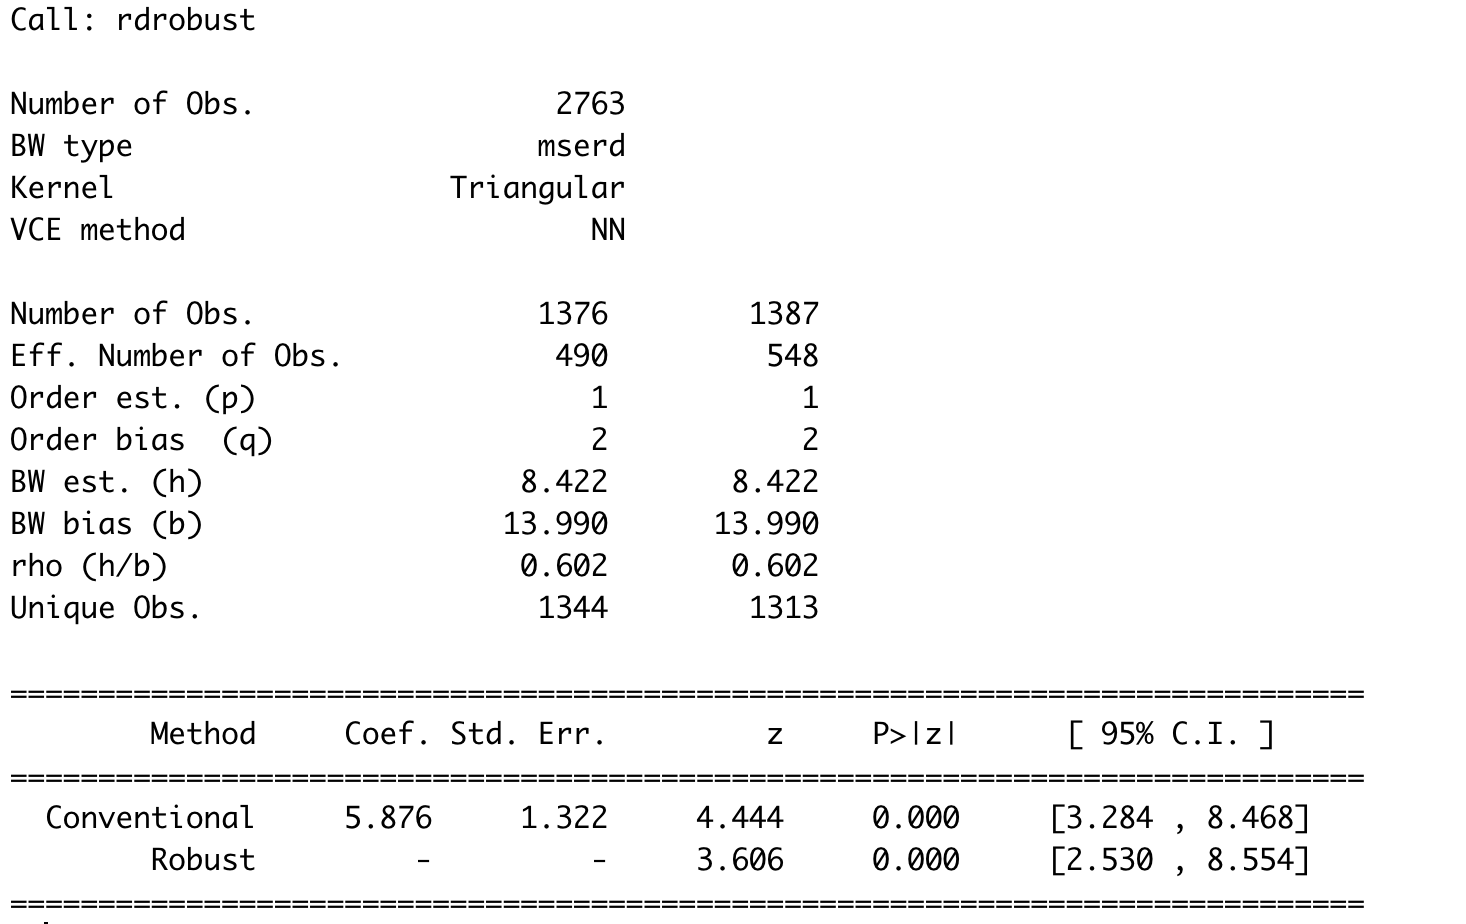
\includegraphics[width=\linewidth]{images/rdrobust_1.png}
      \end{column}%
    \end{columns}
\end{frame}

\begin{frame}{Let's look at it in practice}
    \begin{columns}[onlytextwidth, T] % align columns
      \begin{column}{.6\textwidth}
        \begin{itemize}
        \item Conventional: assumes zero bias in the inference method.
          \begin{itemize}
          \item Coefficient and standard error are standard variance
            estimates that you get from running OLS with chosen $h$
          \item No bias adjustment is done
          \end{itemize}
        \item Robust: accounts for bias in two ways, but \emph{only} in the inference
          \begin{itemize}
          \item Centers CI around the \emph{bias-adjusted} estimate
          \item \emph{Also} accounts for the additional noise from the estimation of the bias term
          \item Can see the steps by using the \texttt{all} option            
          \end{itemize}
        \item<2-> Cattaneo et al. (2020) advocate for:
          \begin{itemize}
          \item Report $\hat{\tau}_{SRD}$ without bias adjustment (it
            is more MSE efficient than the bias corrected estimator)
          \item Report the robust confidence interval
          \end{itemize}
        \end{itemize}
      \end{column}%
      \hfill%
      \begin{column}{.4\textwidth}
        \only<1>{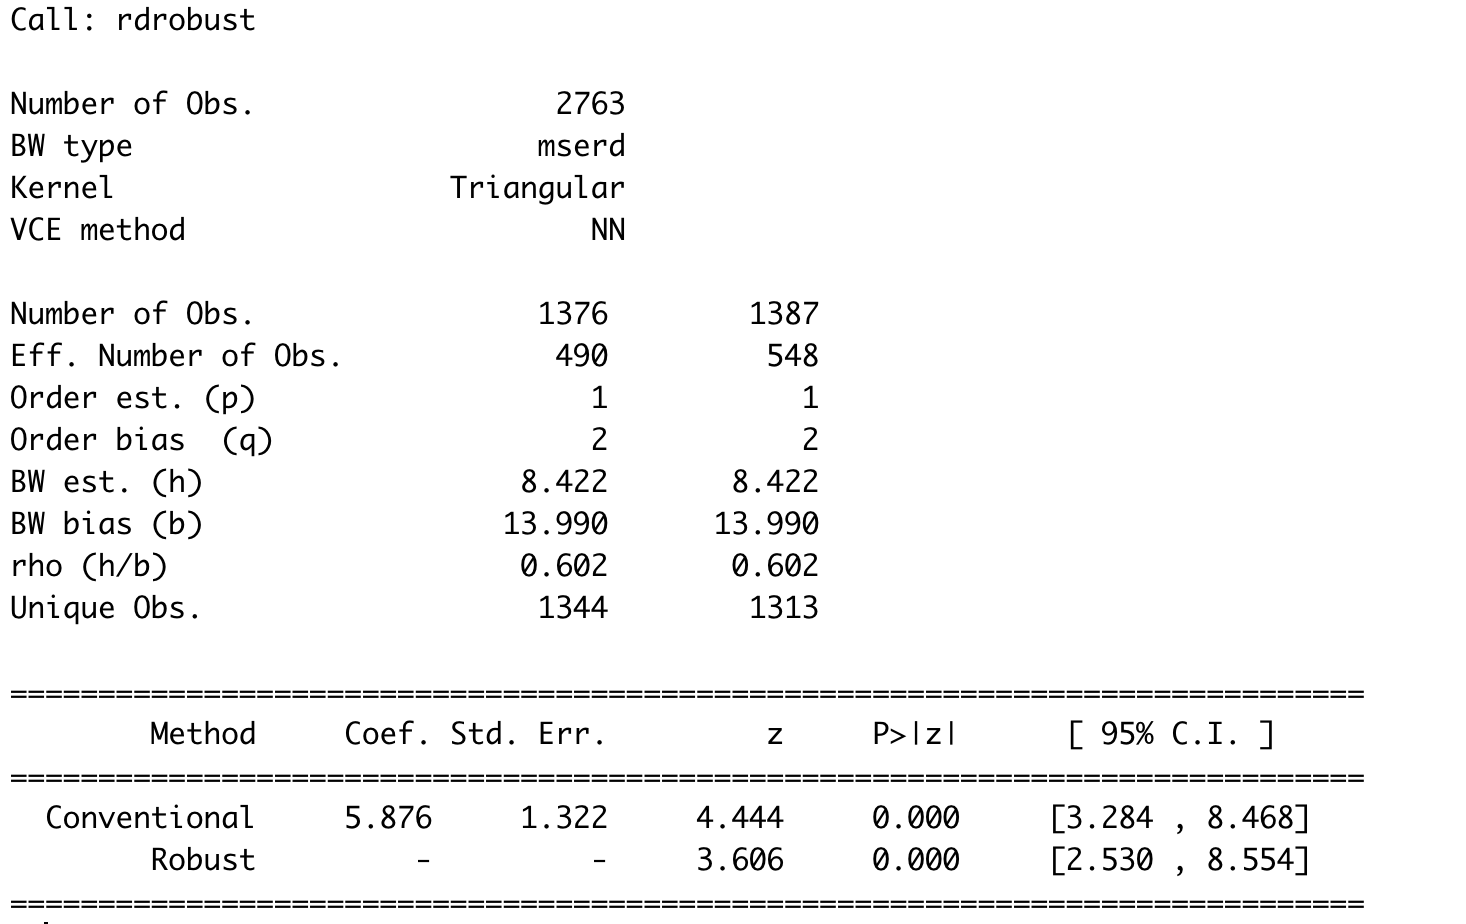
\includegraphics[width=\linewidth]{images/rdrobust_1.png}}
        \only<2>{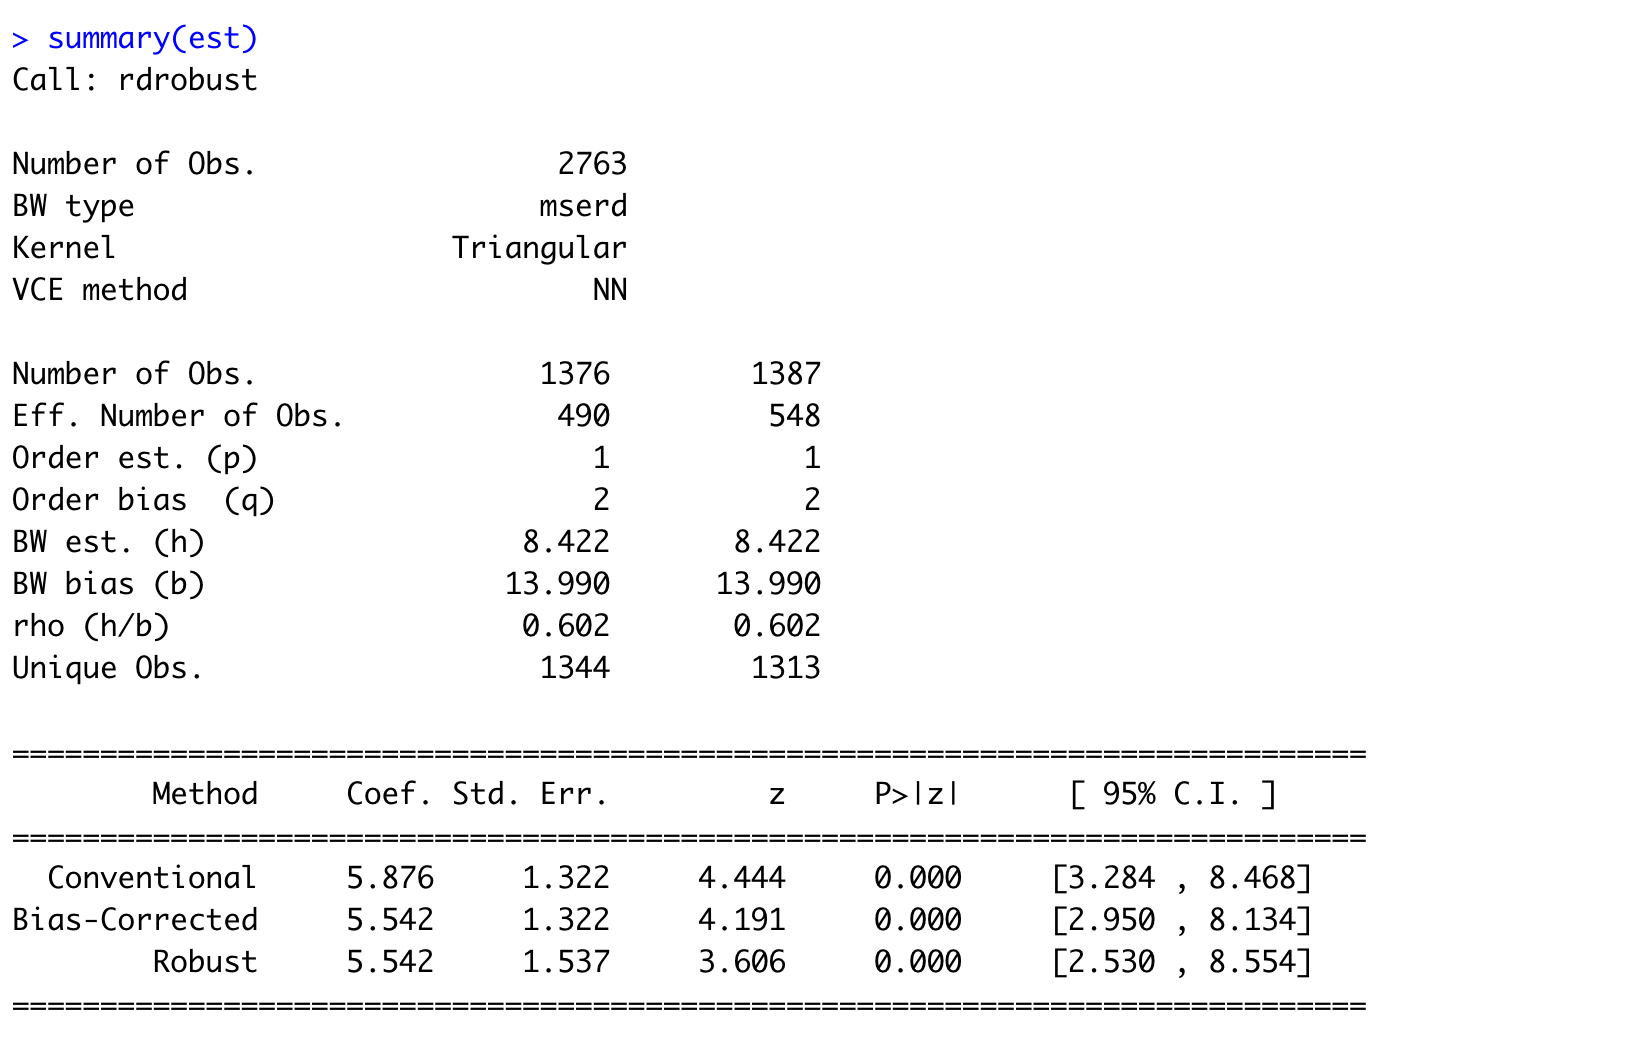
\includegraphics[width=\linewidth]{images/rdrobust_2.png}}        
      \end{column}%
    \end{columns}
\end{frame}

\begin{frame}{What if we can't shrink our bandwidth? Discrete Regression Discontinuity}
    \begin{columns}[onlytextwidth, T] % align columns
      \begin{column}{.6\textwidth}
        \begin{wideitemize}
        \item Bias in the RD estimates comes from the approximation of
          the conditional mean function
          \begin{itemize}
          \item The smaller the bandwidth, the better the local approximation!
          \end{itemize}
        \item What if the running variable is discrete? E.g., age
        \item Kolesar and Rothe (2018) discuss exactly this scenario
          and propose an ``Honest'' RD estimation approach which
          approximates the bias by asssuming a maximum second
          derivative
        \end{wideitemize}
      \end{column}%
      \hfill%
      \begin{column}{.4\textwidth}
        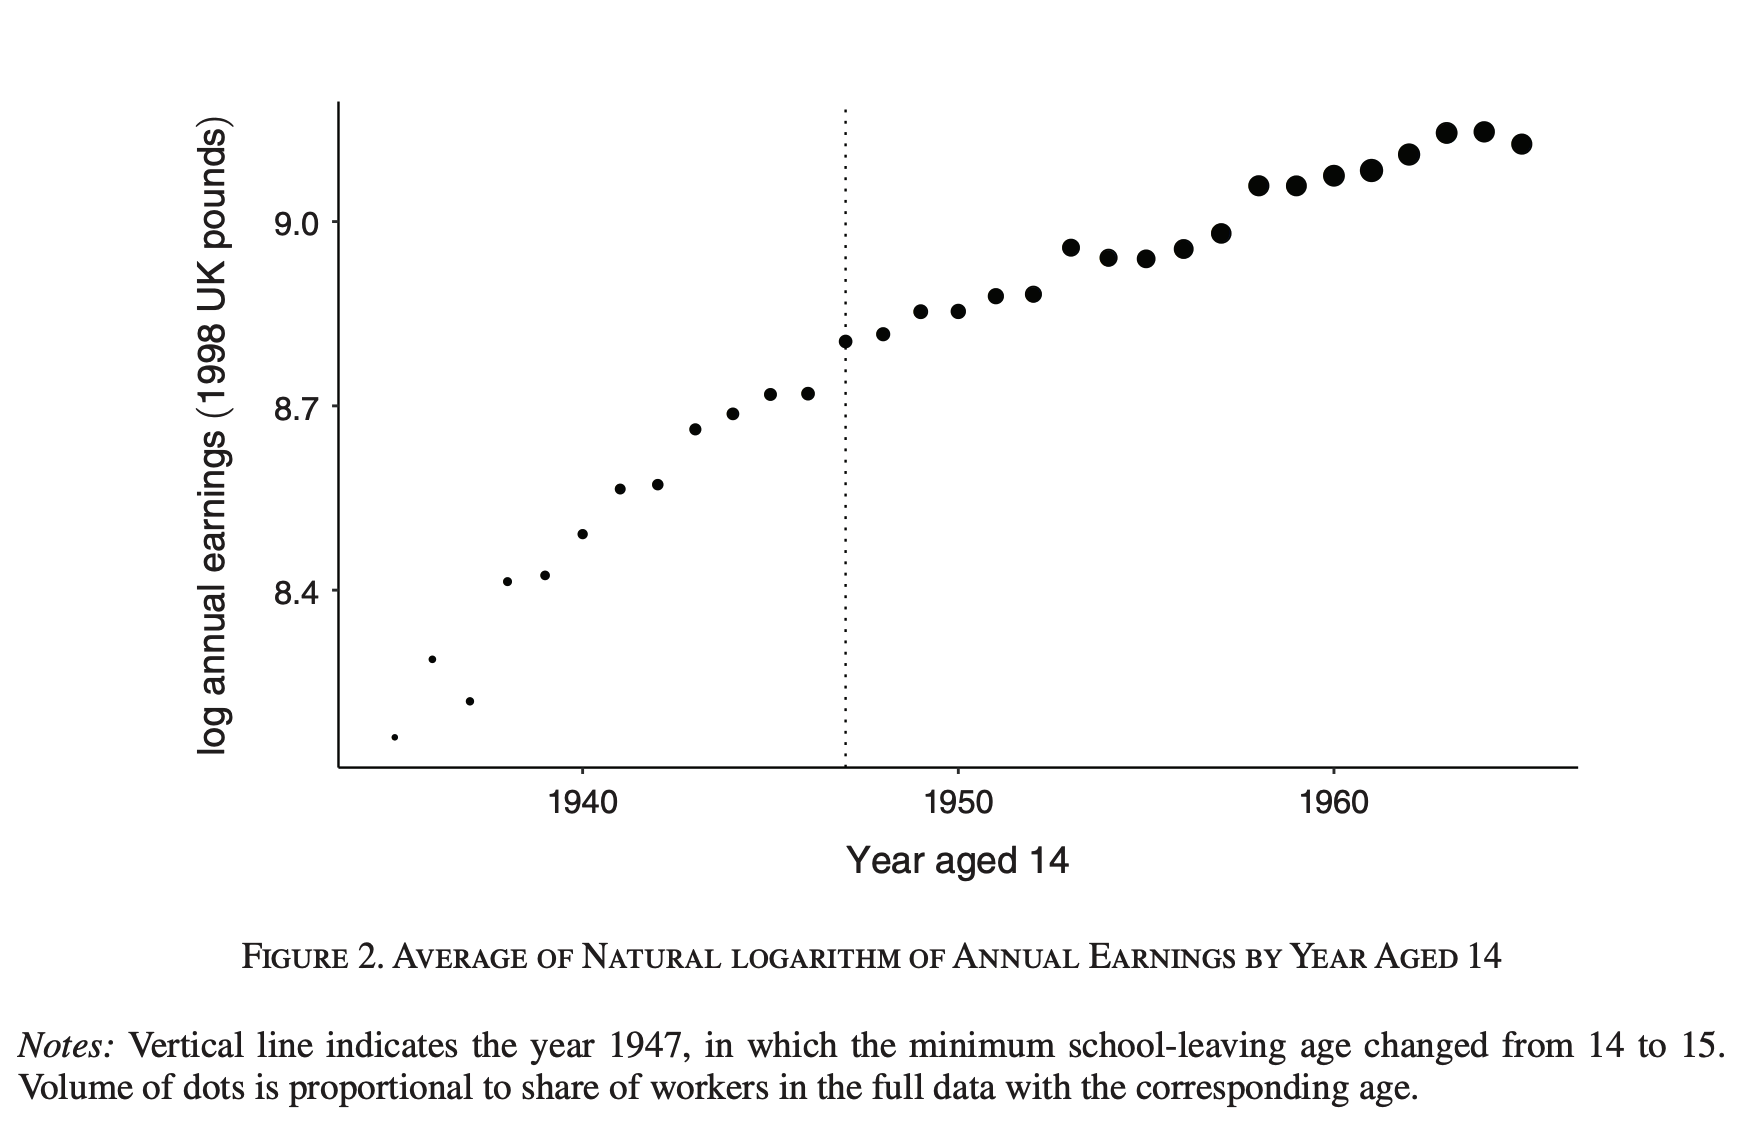
\includegraphics[width=\linewidth]{images/rdhonest_1.png}
      \end{column}%
    \end{columns}
\end{frame}


\begin{frame}{What if we can't shrink our bandwidth? Discrete Regression Discontinuity}
    \begin{columns}[onlytextwidth, T] % align columns
      \begin{column}{.6\textwidth}
        \begin{wideitemize}
        \item Kolesar and Rothe say -- ignore the bias-adjustment
          fact, and just assume undersmoothing. If this is the case,
          you can just use standard Eicker-Huber-White errors
          (e.g. ``robust'' s.e.)
          \begin{itemize}
          \item But we know this argument only works if you can get
            enough observations ``close'' to the cutoff
          \item With discrete variables, this fails
          \end{itemize}
        \item Recall that we're extrapolating the conditional mean function to the cutoff
          \begin{itemize}
          \item If we are willing to put a bound on the 2nd derivative
            function, and assume it is in a class of H\"older
            functions (which is very general), we can bound our
            maximum bias, and use this adjust our confidence intervals
          \end{itemize}
        \end{wideitemize}
      \end{column}%
      \hfill%
      \begin{column}{.4\textwidth}
        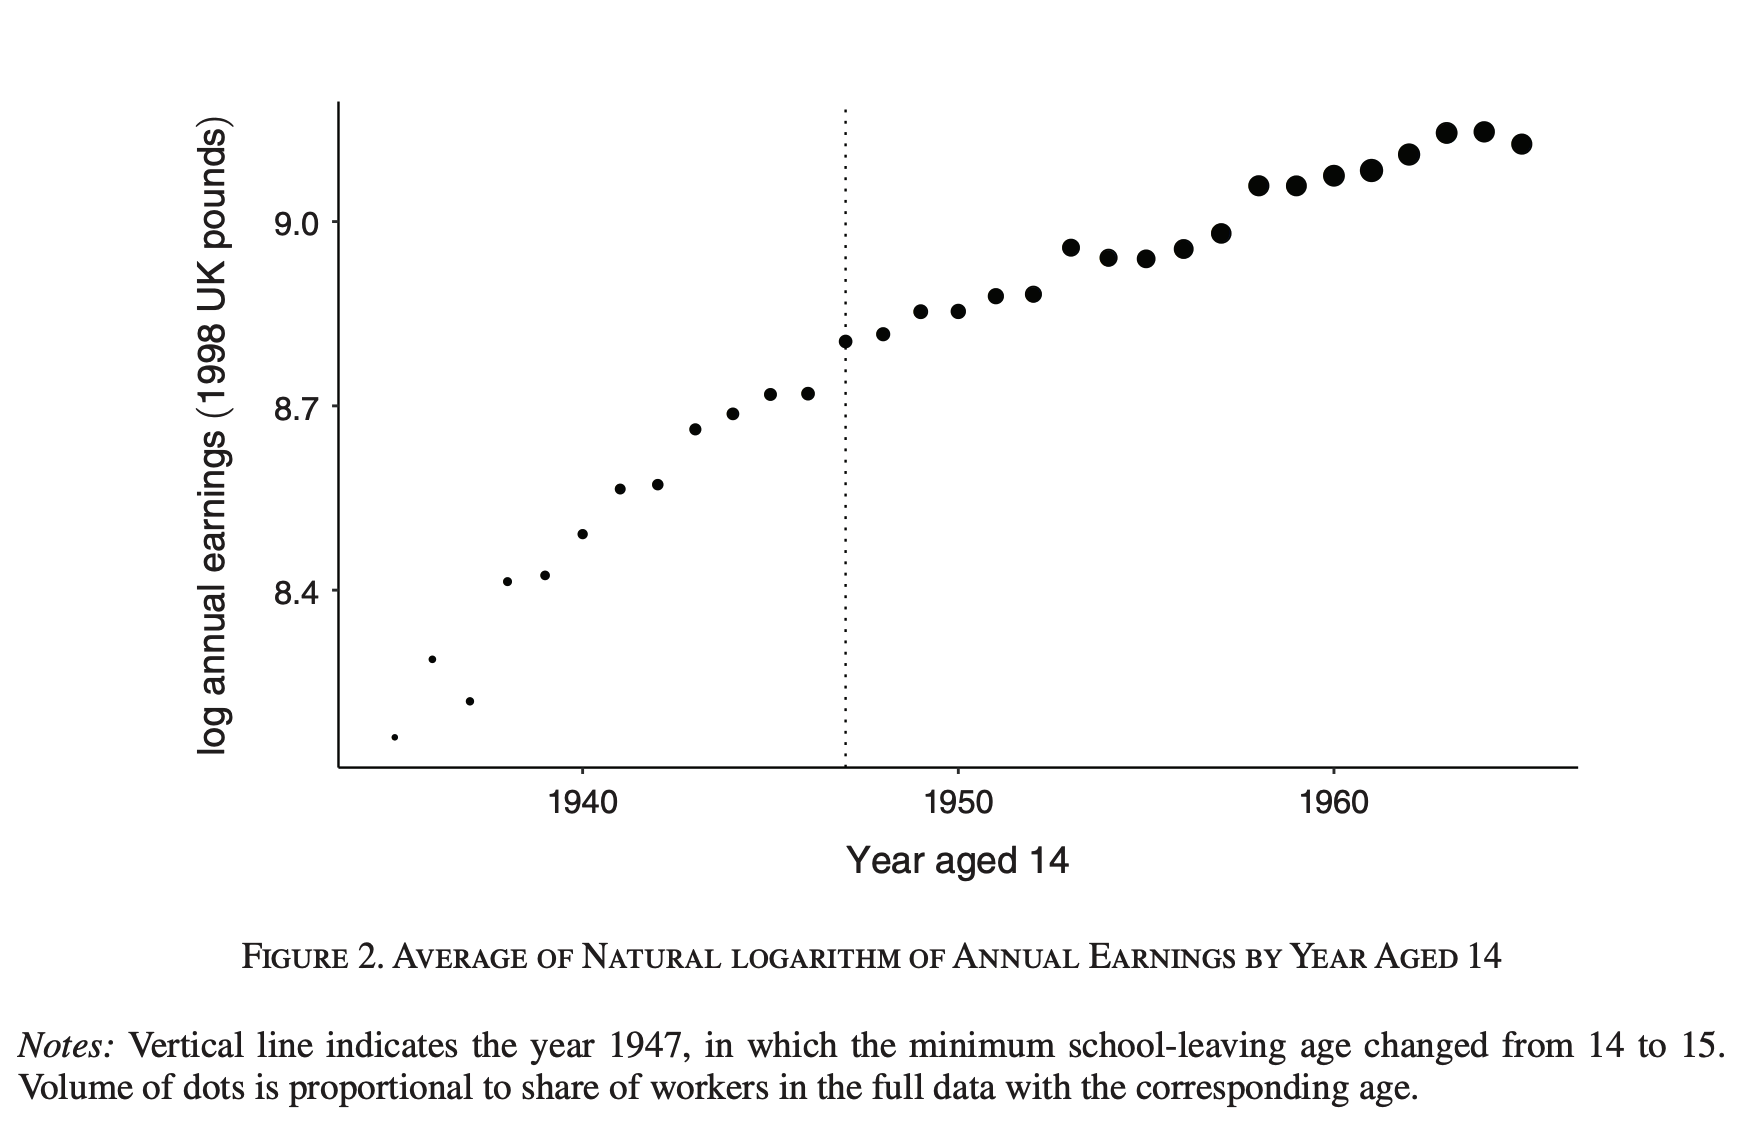
\includegraphics[width=\linewidth]{images/rdhonest_1.png}
      \end{column}%
    \end{columns}
\end{frame}

\begin{frame}{What if we can't shrink our bandwidth? Discrete Regression Discontinuity}
    \begin{columns}[onlytextwidth, T] % align columns
      \begin{column}{.8\textwidth}
        \begin{wideitemize}
        \item This approach is valid even with continuous running
          variables, and is a powerful and robust way to allow for
          misspecification bias
        \item My experience has been that this package
          (\texttt{RDHonest}) works much better with discrete RV than
          \texttt{rdrobust} (which has adjustments for discreteness)
        \item However, you need to choose your maximum bias, and it
          can be challenging to do so \emph{ex ante}.
          \begin{itemize}
          \item Armstrong and Kolesar discuss ways to do this in a
            data driven way given additional assumptions.
          \item You should also show how your results change with this
            parameter choice, similar to bandwidth!
          \end{itemize}
        \end{wideitemize}
      \end{column}%
      \hfill%
      \begin{column}{.4\textwidth}
      \end{column}%
    \end{columns}
\end{frame}

\begin{frame}{Comparing RDHonest and rdrobust}
    \begin{columns}[onlytextwidth, T] % align columns
      \begin{column}{.3\textwidth}
        \begin{wideitemize}
        \item First, let's look at the plot
        \item RDRobust estimate is 5.9 (2.5,8.5)
        \item RDHonest estimate varies depending on choice of second
          derivative bound. For $M=0.1$: 5.9 (2.9, 8.8)
        \item What would you pick for $M$?
        \end{wideitemize}
      \end{column}%
      \hfill%
      \begin{column}{.7\textwidth}
        \only<1>{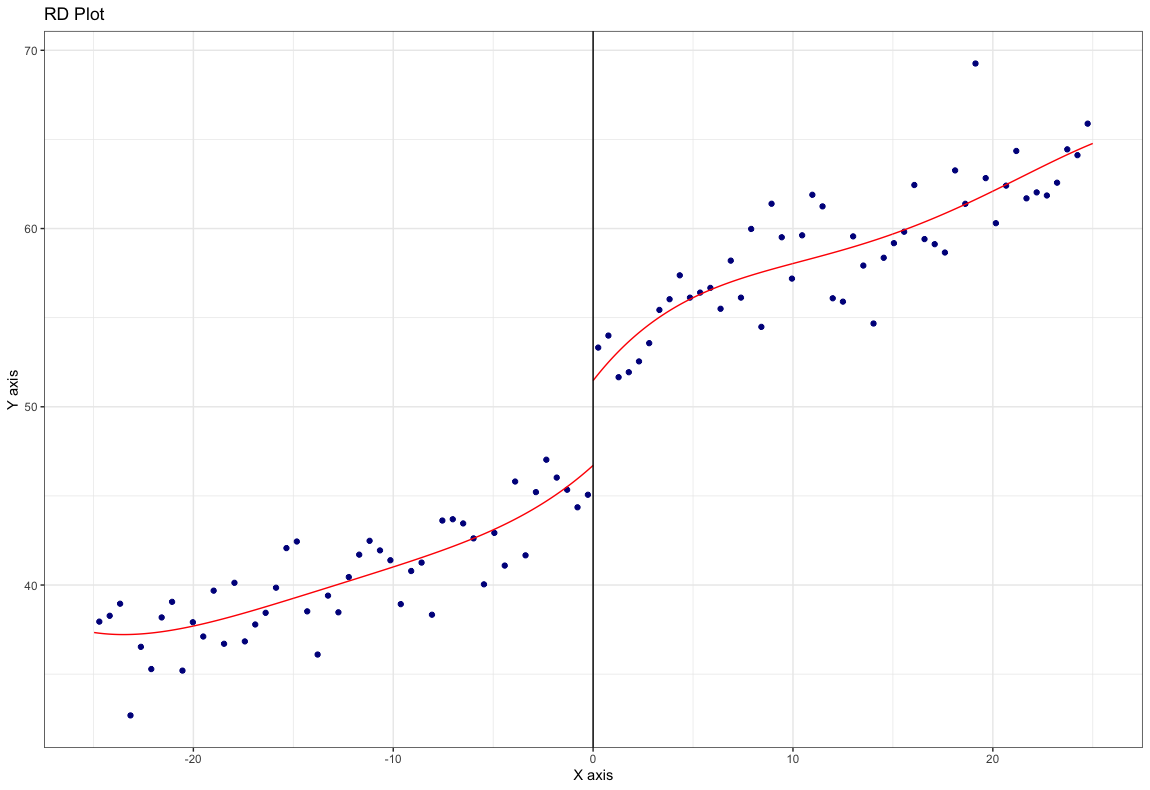
\includegraphics[width=\linewidth]{images/rdplot_lee.png}}
        \only<2>{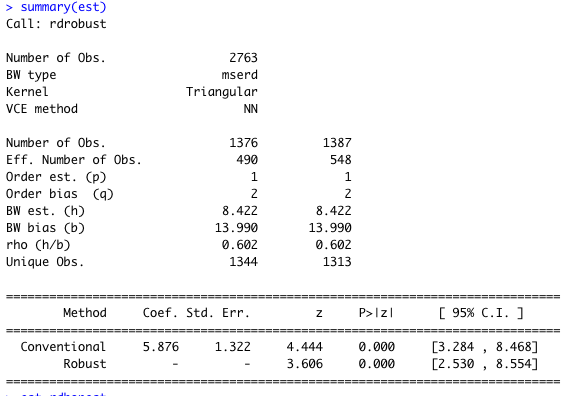
\includegraphics[width=\linewidth]{images/rdrobust_est_lee.png}}
        \only<3>{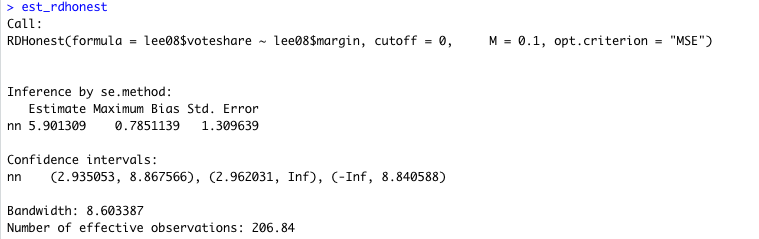
\includegraphics[width=\linewidth]{images/rdhonest_est_lee_M1.png}}
        \only<4>{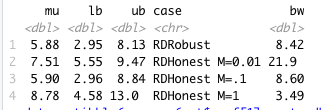
\includegraphics[width=\linewidth]{images/cases_rd.png}}                
      \end{column}%
    \end{columns}
\end{frame}



\begin{frame}{What if we can't shrink our bandwidth? Discrete Regression Discontinuity}
    \begin{columns}[onlytextwidth, T] % align columns
      \begin{column}{.6\textwidth}
        \begin{wideitemize}
        \item Another similar paper in this space is Imbens and Wager
          (2019)
          \begin{itemize}
          \item The estimation approach also puts bound on the second
            derivative, but uses a numerical approach to do estimation
          \item Package in R: \texttt{optrdd}
          \end{itemize}
        \item This approach potentially has slightly smaller confidence intervals
        \item It also generalizes to multivariate RD settings
          (e.g. spatial settings) quite easily
          \begin{itemize}
          \item See also \texttt{rdmulti}, which also allows for multiple cutoffs
          \end{itemize}
        \end{wideitemize}
      \end{column}%
      \hfill%
      \begin{column}{.4\textwidth}
        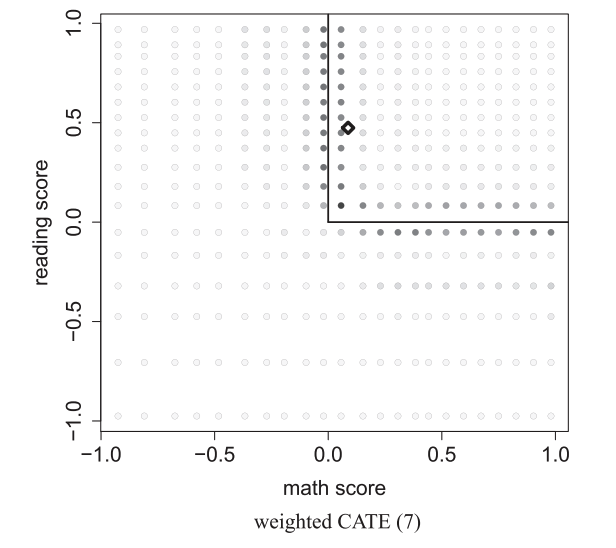
\includegraphics[width=\linewidth]{images/rd_imbenswager.png}
      \end{column}%
    \end{columns}
\end{frame}

\begin{frame}{Multiple Cutoffs}
    \begin{columns}[onlytextwidth, T] % align columns
      \begin{column}{.6\textwidth}
  \begin{wideitemize}
  \item Cattaneo, Titiunik, Vazquez-Bare and Keele (2016) and Bertanha
    (2020) touch on what to do when not every threshold is the same
    (See the discussion in Cattaneo, Idrobo and Titiunik's extensions
    textbook for a very clean discussion)
    \begin{itemize} 
    \item E.g. \textbf{MultiThreshold} contrast a political election with 2 vs. 3 candidates
      -- what is the ``winning'' threshold?
    \item E.g. \textbf{MultiCutoff} Cutoff based on two test scores
    \end{itemize}
  \item These have separate complications associated with them
  \end{wideitemize}
  \end{column}
      \begin{column}{.4\textwidth}
        \only<1>{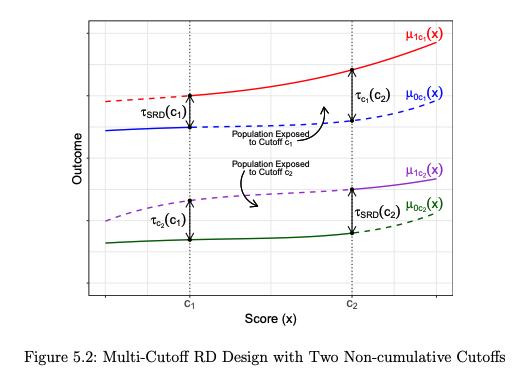
\includegraphics[width=\linewidth]{images/multicutoff.png}}
        \only<2>{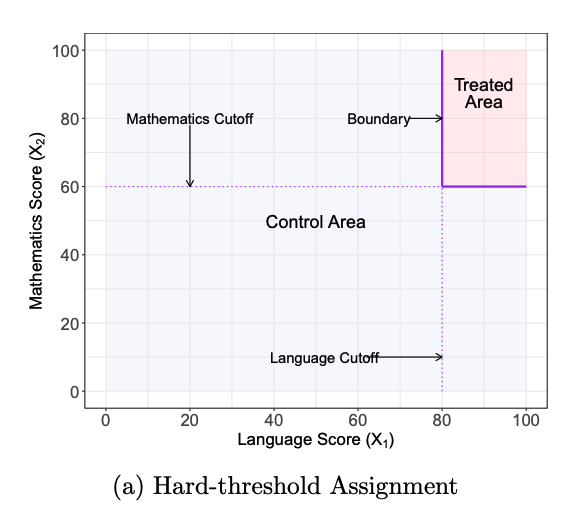
\includegraphics[width=\linewidth]{images/multiscore.png}}        
      \end{column}%
    \end{columns}
\end{frame}

\begin{frame}{Multiple Threshold - Cumulative vs. Not}
    \begin{columns}[onlytextwidth, T] % align columns
      \begin{column}{.6\textwidth}
  \begin{wideitemize}
  \item Do the treatment cutoffs vary based on unit, or are there just many of them?
  \item An example non-cumulative case is when the thresholds vary on
    geography: all units could potentially be exposed to treatments
    defined at different cutoffs
  \item An example cumulative case is where dosing is a function of
    the score -- those facing different treatment cutoffs are not
    comparable (e.g. a support problem in the running variable)
  \end{wideitemize}
  \end{column}
      \begin{column}{.4\textwidth}
        \only<1>{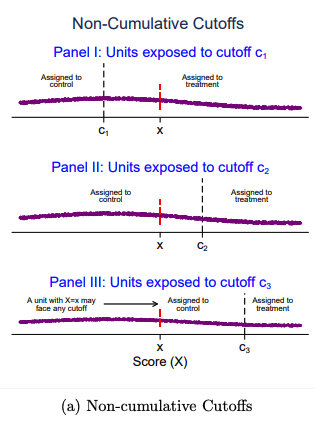
\includegraphics[width=\linewidth]{images/cutoff_noncum.png}}
        \only<2>{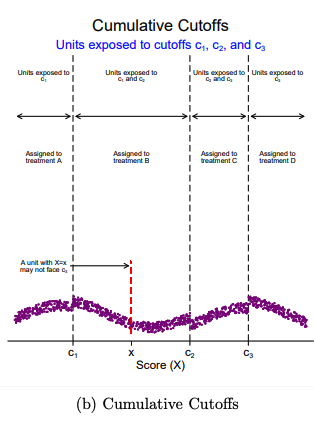
\includegraphics[width=\linewidth]{images/cutoff_cum.png}}        
      \end{column}%
    \end{columns}
\end{frame}


\begin{frame}{Multiple Threshold - Non-cumulative pooling}
  \begin{columns}[onlytextwidth, T] % align columns
    \begin{column}{.6\textwidth}
      \begin{wideitemize}
      \item With non-cumulative treatments, can consider a cutoff specific
        treatment and proceed identically -- each one identified separately
      \item To pool these estiamtes, you can normalize and center at the same point
        \begin{equation}
          \tau_{SRD}^{pool} = \sum_{c} w(c) \tau_{SRD}(c), \; w(c) = \frac{f_{X|C}(c|c) Pr(C = c)}{\sum_{c}f_{X|C}(c|c) Pr(C = c)}
        \end{equation}
      \end{wideitemize}
    \end{column}
    \begin{column}{.4\textwidth}
      \only<1>{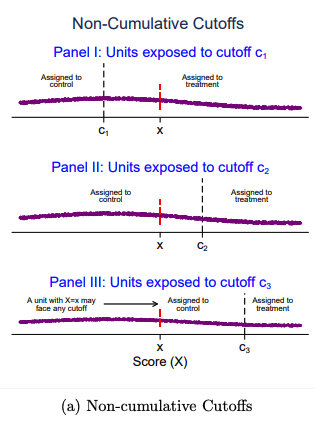
\includegraphics[width=\linewidth]{images/cutoff_noncum.png}}
    \end{column}%
  \end{columns}
\end{frame}

\begin{frame}{Multiple Cutoffs}
  \begin{columns}[onlytextwidth, T] % align columns
    \begin{column}{.6\textwidth}
      \begin{wideitemize}
      \item With multiple scores, the limits are defined in a multi-dimensional way.
      \item Integrating over these points has a similar logic to multiple-threshold
      \end{wideitemize}
    \end{column}
    \begin{column}{.4\textwidth}
      \only<1>{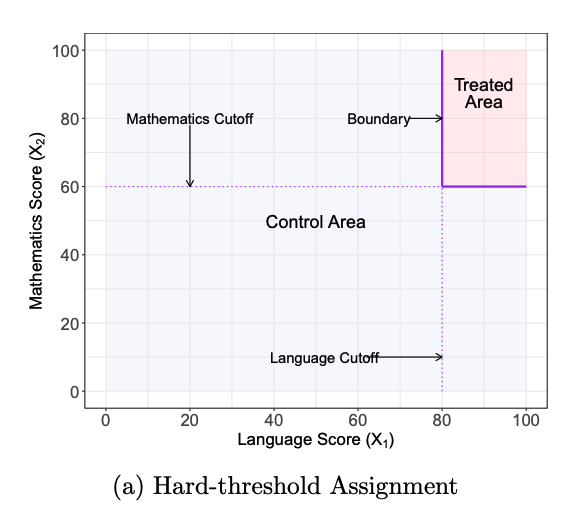
\includegraphics[width=\linewidth]{images/multiscore.png}}
    \end{column}%
  \end{columns}
\end{frame}


\begin{frame}{What about bunching? Bounds on Treatment effects}
    \begin{columns}[onlytextwidth, T] % align columns
      \begin{column}{.6\textwidth}
        \begin{wideitemize}
        \item Recall our Mcrary (2008) test for bunching in the running variable
          \begin{itemize}
          \item Concern is  maniuplated running variable
          \end{itemize}
        \item For example, in Dee et al. (2019), there is clear
          manipulation, and so using this RD directly would be
          spurious
        \item This is a particularly egregious case -- many are less stark
          \begin{itemize}
          \item Moreover, you may also be underpowered to detect the
            break if they do exist!
          \end{itemize}
        \end{wideitemize}
      \end{column}%
      \hfill%
      \begin{column}{.4\textwidth}
        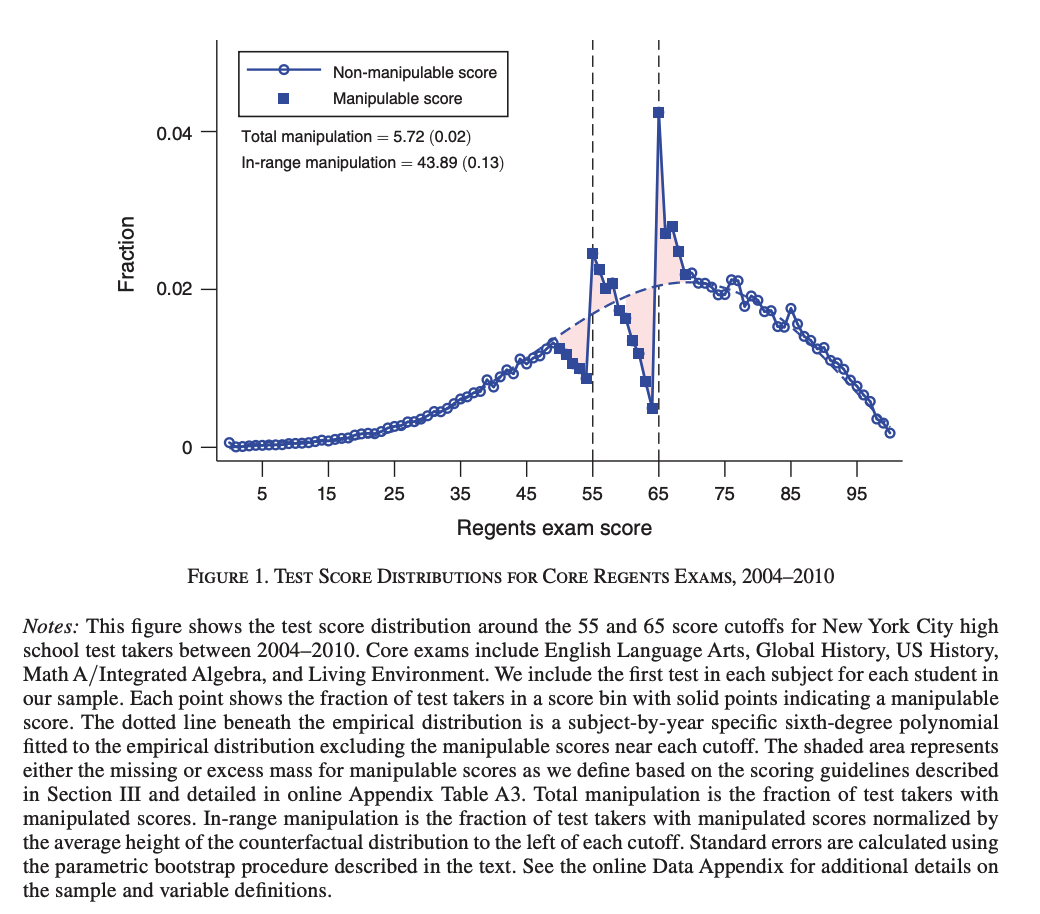
\includegraphics[width=\linewidth]{images/dee_dobbie.png}
      \end{column}%
    \end{columns}  
  \end{frame}


  \begin{frame}{What about bunching? Bounds on Treatment effects}
    \begin{columns}[onlytextwidth, T] % align columns
      \begin{column}{\textwidth}
        \begin{itemize}
        \item Gerard, Rokkanen and Rothe (2020) propose a partial
          identification approach to allow for the possibility of
          bunching
        \item Think of this as a check on the robustness of the
          results -- how sensitive are the results to manipulation?
          \begin{itemize}
          \item Code is available for R and Stata: \texttt{rdbounds}
          \end{itemize}
        \item The key result hinges on the idea that the manipulation
          goes in one direction, and that these right-ward
          manipulated individuals ``mask'' the true underlying effect
          \begin{itemize}
          \item These individuals are always manipulated to the right
            side of the cutoff (they are the ``excess mass'')
          \end{itemize}
        \item Derive sharp bounds for those individuals who can
            actually be affected by the treatment
          \begin{itemize}
          \item Do this by identifying the share of the ``masking'' individuals: $\tau = 1- f_{Z}(0^{-})/f_{Z}(0^{+})$.
          \item If Mcrary test holds, this number is zero!
          \end{itemize}
        \item This is a very nice approach if you have bunching issues in your design
        \end{itemize}
      \end{column}%
      \hfill%
      \begin{column}{.4\textwidth}
      \end{column}%
    \end{columns}
\end{frame}

\begin{frame}{An important question}
  \begin{wideitemize}
  \item Imagine you have an RD that you ran, and you want to compare
    across estimates across two groups ($W_{i} \in (0,1)$)
    \begin{itemize}
    \item How would you do this?
    \end{itemize}
  \item Note how you would do it in a simple OLS setting:
    \begin{align*}
      y_{i} &= \alpha_{0} +  Z_{i}\gamma_{0} + Z_{i}1(Z_{i} > 0)\delta_{0} + 1(Z_{i} > 0)\tau_{SRD} \\
            &+ W_{i}\alpha_{1} +  W_{i}Z_{i}\gamma_{0} + W_{i}Z_{i}1(Z_{i} > 0)\delta_{0} + W_{i}1(Z_{i} > 0)\tau_{SRD,diff} + \epsilon_{i}
    \end{align*}
              
    $\tau_{SRD,diff}$ would give you the difference -- this approach
    is easy if you pick a bandwidth and use a uniform kernel
  \item But now we have all these better tools (and we need them in a
    lot of places) -- how could still do this?
    \begin{itemize}
    \item  Apply the delta method to the transformation we want to do!
    \end{itemize}
    
  \end{wideitemize}
\end{frame}

\begin{frame}{Comparing coefficients across setups}
  \begin{wideitemize}
  \item Consider an RDRobust estimate for $\tau(W=1)$ and $\tau(W=0)$. 
    \begin{itemize}
    \item The difference is $f(\tau_{1}, \tau_{0}) = \tau_{1} - \tau_{0}$
    \end{itemize}
  \item Recall that our variance estimate is $(f')^{T}\Sigma f'$,
    where $f'$ is the gradient vector and $\Sigma$ is our variance
    covariance matrix of $\tau_{1}$ and $\tau_{0}$.
    \begin{itemize}
    \item How do we get $\Sigma$? Well, recall that we estimated these
      separately from one another, so the covariance terms are zero
    \item Hence, $\Sigma$ is just the
      $\text{diag}(Var(\tau_{1}), Var(\tau_{0}))$
    \end{itemize}
  \item In our simple example, $Var(\tau_{1} - \tau_{0}) = Var(\tau_{1}) + Var(\tau_{0})$ and so Delta method is exact
    \begin{itemize}
    \item However, can study more complicated functions as well!
    \item This approach also works with the \texttt{RDHonest} approach
      as well, just need to account for the additional bias terms (see
      Appendix of Armstrong and Kolesar (2020))
    \end{itemize}
  \end{wideitemize}
\end{frame}

\begin{frame}{Regression Kink Design}
    \begin{columns}[onlytextwidth, T] % align columns
      \begin{column}{.6\textwidth}
        \begin{wideitemize}
        \item Much of our discussion centered around a discontinuous
          jump in the outcome (and treatment variable)
        \item Nielsen et al. (2010) initially coin the concept instead
          of a regression kink design (further worked on by Card, Lee,
          Pei and Weber (2016)
          \begin{itemize}
          \item Key difference here exploits a difference in
            \emph{slope}, rather than a level difference
          \item Technically, could be both!
          \end{itemize}
        \item This approach is very powerful because many policy tools
          have linear shifts in incentives, rather than jumps
        \end{wideitemize}
      \end{column}%
      \hfill%
      \begin{column}{.4\textwidth}
        \only<1>{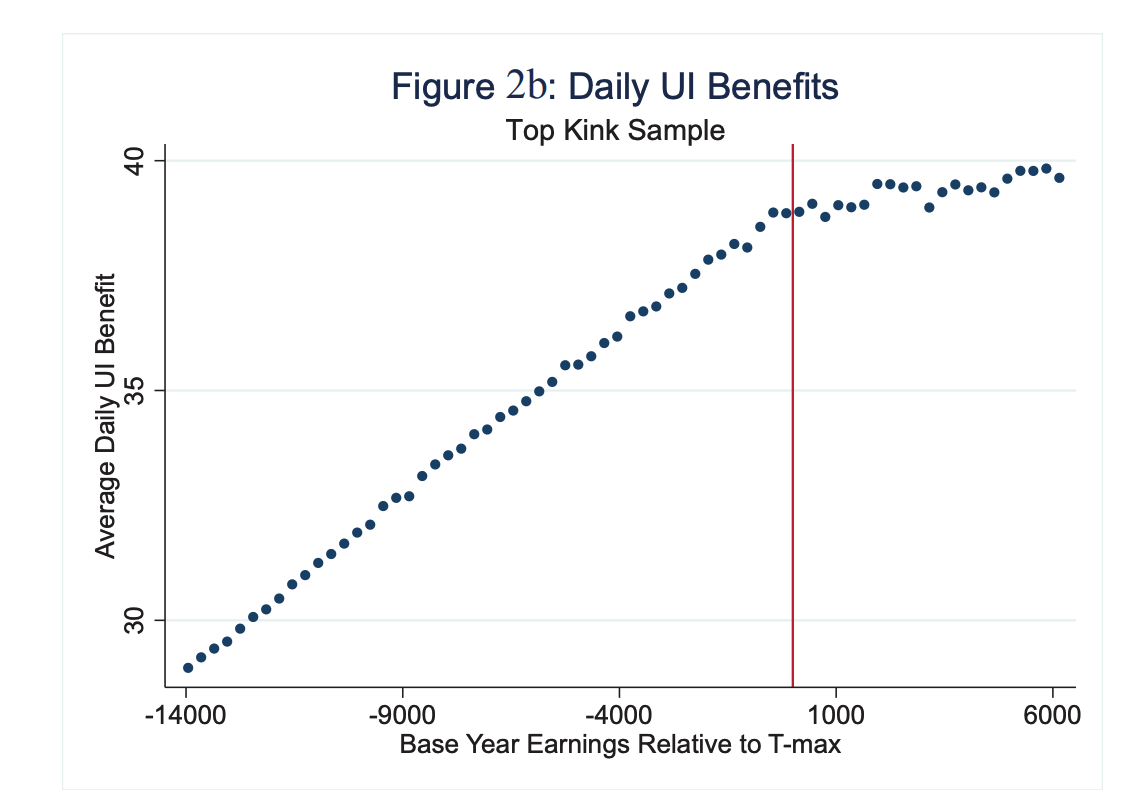
\includegraphics[width=\linewidth]{images/card_rkd.png}}
        \only<2>{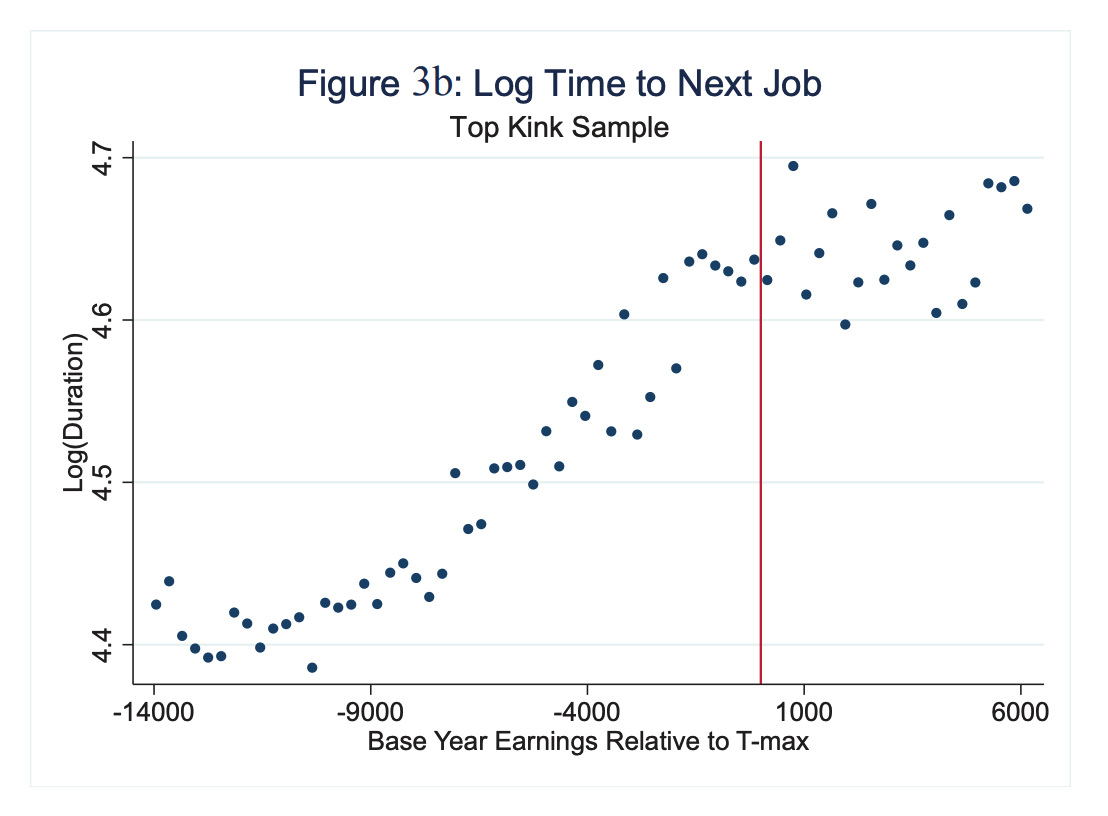
\includegraphics[width=\linewidth]{images/card_rkd2.png}}        
      \end{column}%
    \end{columns}  
\end{frame}


\begin{frame}{Regression Kink Design}
    \begin{columns}[onlytextwidth, T] % align columns
      \begin{column}{.6\textwidth}
        \begin{wideitemize}
        \item This is a deeply interesting approach, but requires a \emph{lot} of data
        \item Why? because slope changes are hard to see. Did the
          slope change because of curvature, of because of a kink?
        \item Ganong and J\"ager (2018) discuss a test for this to
          account for this fact
        \item This is a good approach to keep in mind! See, e.g.,
          Indarte (2021)
        \end{wideitemize}
      \end{column}%
      \hfill%
      \begin{column}{.4\textwidth}
        \only<1>{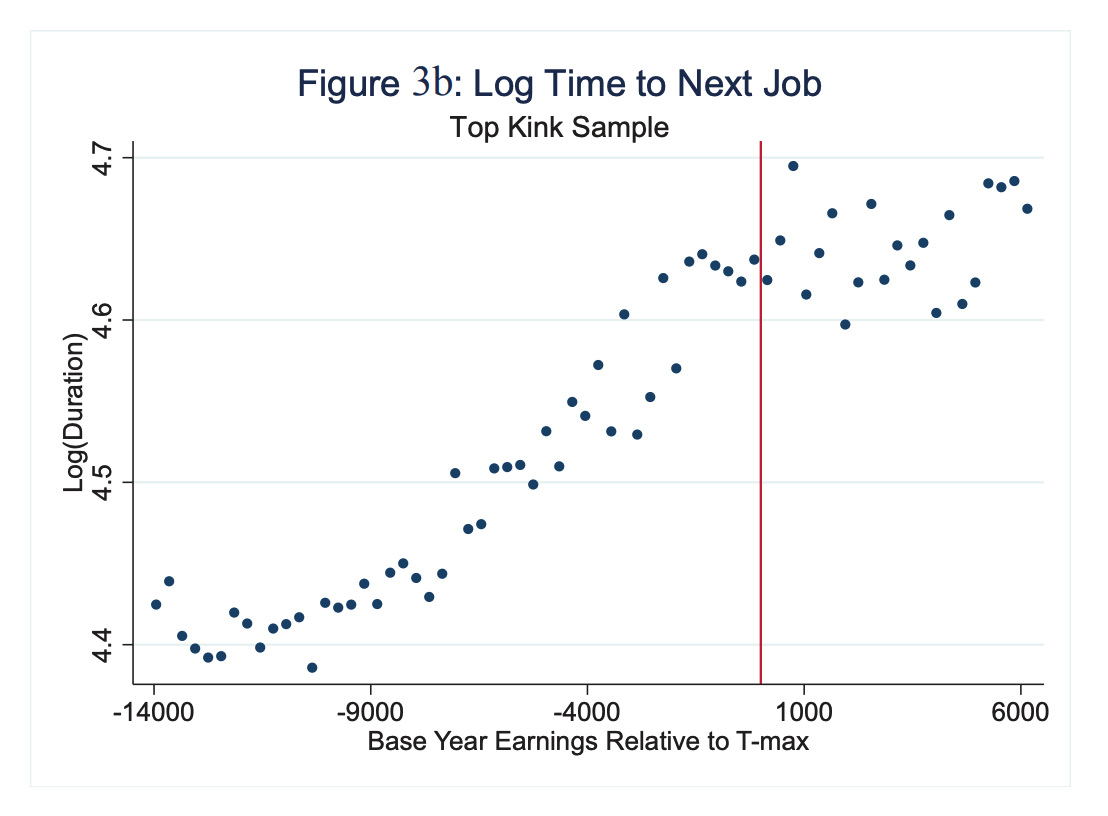
\includegraphics[width=\linewidth]{images/card_rkd2.png}}
        \only<2>{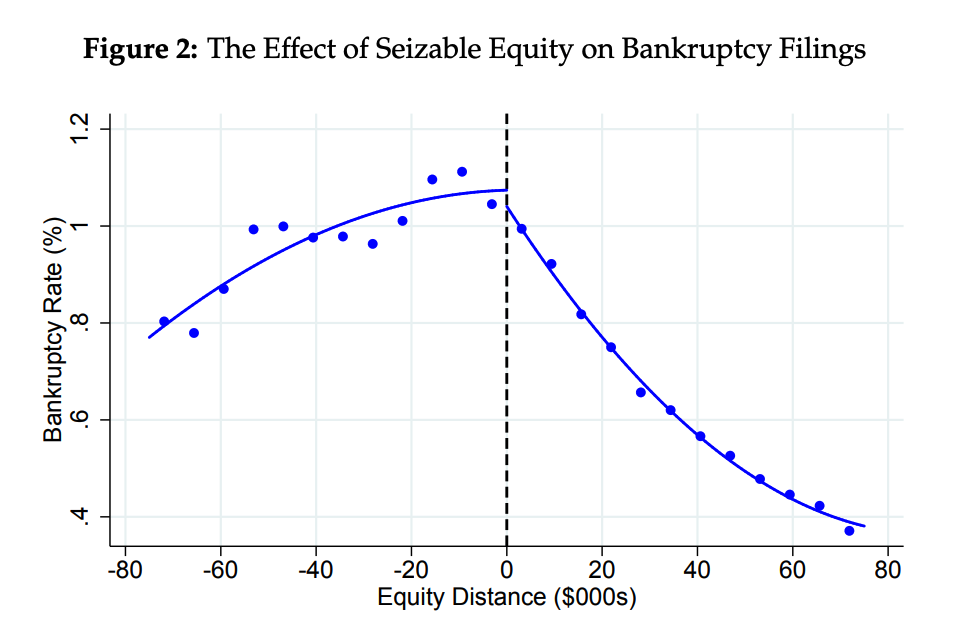
\includegraphics[width=\linewidth]{images/indarte.png}}                
      \end{column}%
    \end{columns}  
\end{frame}







\end{document}